\documentclass{article}
\usepackage[utf8]{inputenc}
\usepackage{graphicx}
\usepackage[T1]{fontenc}
\usepackage[italian]{babel}
\usepackage{hyphenat}
\usepackage{url}
\usepackage{setspace}
\usepackage{parskip}
\usepackage{hyperref}
\usepackage{framed}
\usepackage{array}
\usepackage{listings}
\usepackage{makecell}
\graphicspath{{images/}}
\lstset{language=C,basicstyle=\ttfamily,
commentstyle=\color{green}\ttfamily,
keywordstyle=\color{blue}}
\begin{document}
\begin{titlepage}
    \begin{center}
        \vspace*{1cm}
        
        \sffamily{{\Huge  Progetto di Sistemi Operativi}}
        
        \vspace{0.5cm}
     {\Large \sffamily{Uno schema di coordinamento vagamente ispirato alla 
    Movement Authority per ERTMS/ETCS LV 1 e LV 2 }}
        
        \vspace{0.5cm}
    
      \large Anno accademico 2022/2023
    \vspace{0.5cm}
    
    Data di consegna: 00/00/0000
    
    \vspace{0.5cm}
    \large{\textbf{Aliaksei Shapiolkin} \\Matricola: 6666666\\Email: \href{          
         mailto: aliaksei.shapiolkin@stud.unifi.it}{aliaksei.shapiolkin@stud.unifi.it}
    
    \textbf{Andrea Toti}\\Matricola: 6367319\\Email: \href{mailto:andrea.toti@stud.unifi.it}{andrea.toti@stud.unifi.it} 
    }
      \vspace{0.2cm}
      \vspace{0.7cm}
        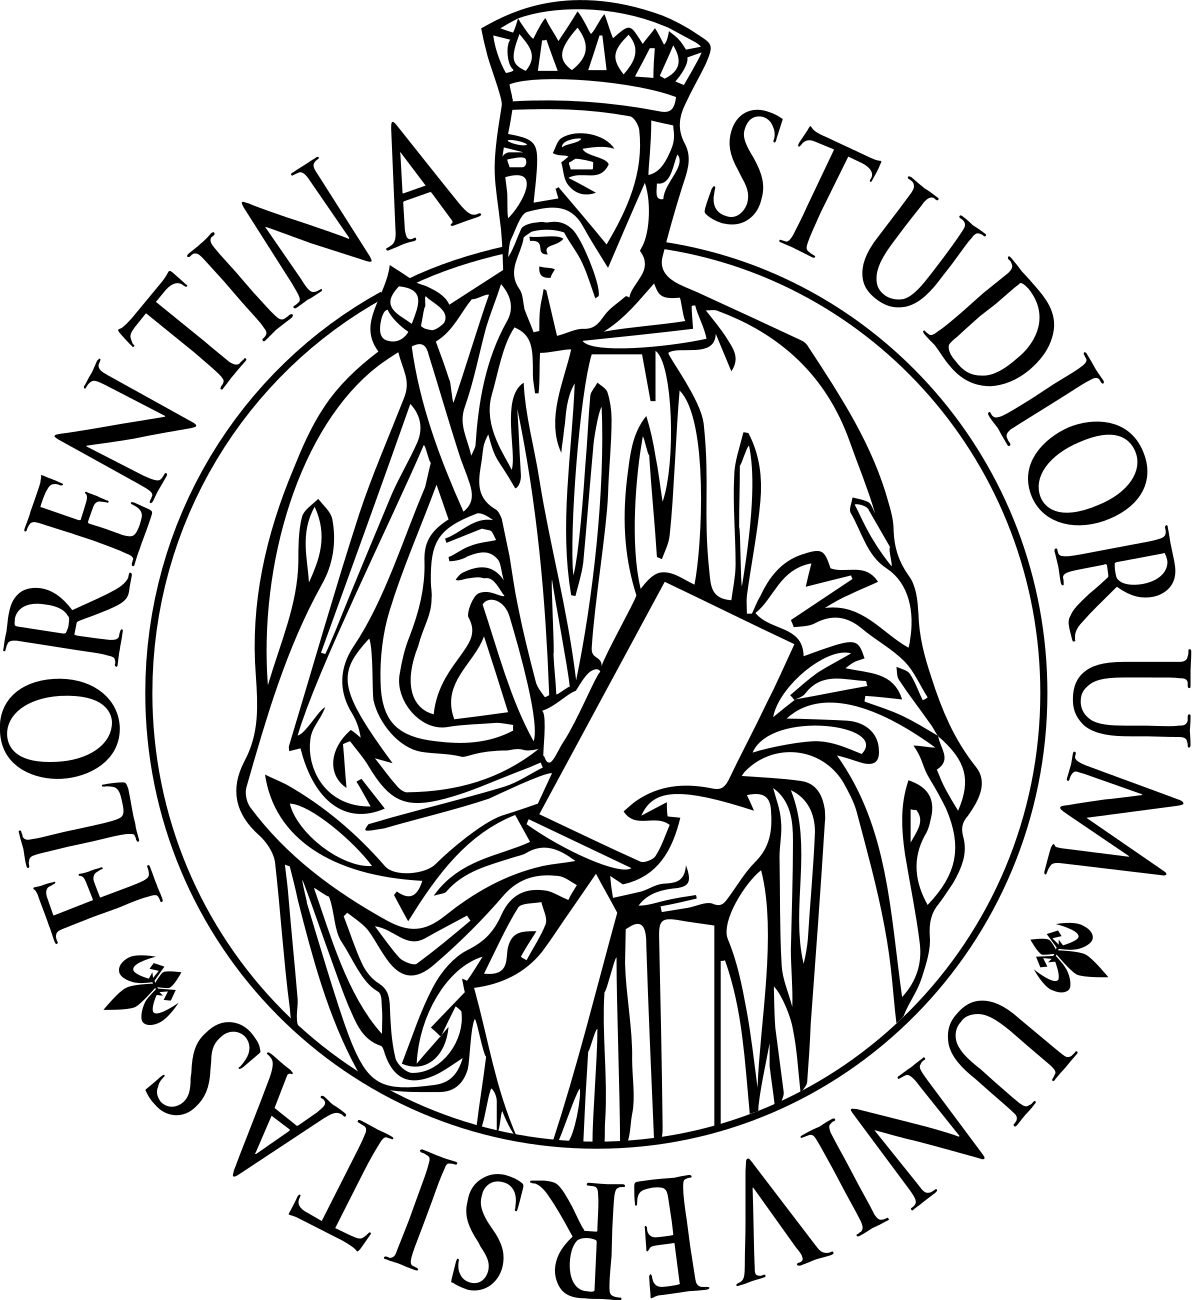
\includegraphics[width=0.55\textwidth]{logo.png} 
    \end{center}
    \end{titlepage}
    
\tableofcontents
\section{Elementi opzionali}
\begin{table}[h]
\centering
    \begin{tabular}{ |c|c|c| } 
 \hline
\textsf{\textbf{Elemento facoltativo}} & \textsf{\textbf{Realizzato}} & \textsf{\textbf{Descrizione metodo}} \\ 
 \hline
 \makecell {Implementare soluzioni per gestire\\ letture e scritture concorrenti} & SI &  \\ 
 \hline
 \makecell{In caso di informazione
 discordante tra RBC\\ e boe, il
 TRENO rimane fermo} & SI/NO &  \\ 
 \hline
 \makecell{terminazione di PADRE\_TRENI e \\PROCESSO\_TRENO basata sul segnale SIGUSR1}&SI&\\
\hline
\makecell{Terminazione di RBC basata sul
segnale SIGUSR2}&SI& \\[0.5ex]
\hline
\end{tabular}
\end{table}
\end{document}
